%% tags: [recurrence relations]
%% source: 2023-fa-midterm_01
\begin{prob}[(2 points)]
    Solve the below recurrence, stating the solution in asymptotic notation. Show your work.
    \[
        T(n) =
        \begin{cases}
            T(n/2) + \Theta(n) & n > 1 \\
            \Theta(1) & n = 1
        \end{cases}
    \]

    \begin{soln}{4.5in}
        $\Theta(n)$.

        Unrolling several times, we find:

        
\includegraphics[width=.1\textwidth]{plot1.png}

        On the $k$th unroll, we'll get:
        \[
            T(n) = T(n/2^k) + \left[
                n + \frac{n}{2} + \frac{n}{4} + \ldots + \frac{n}{2^{k-1}}
            \right]
        \]

        It will take $\log_2 n$ unrolls to each the base case. Substituting this for
        $k$, we get:

        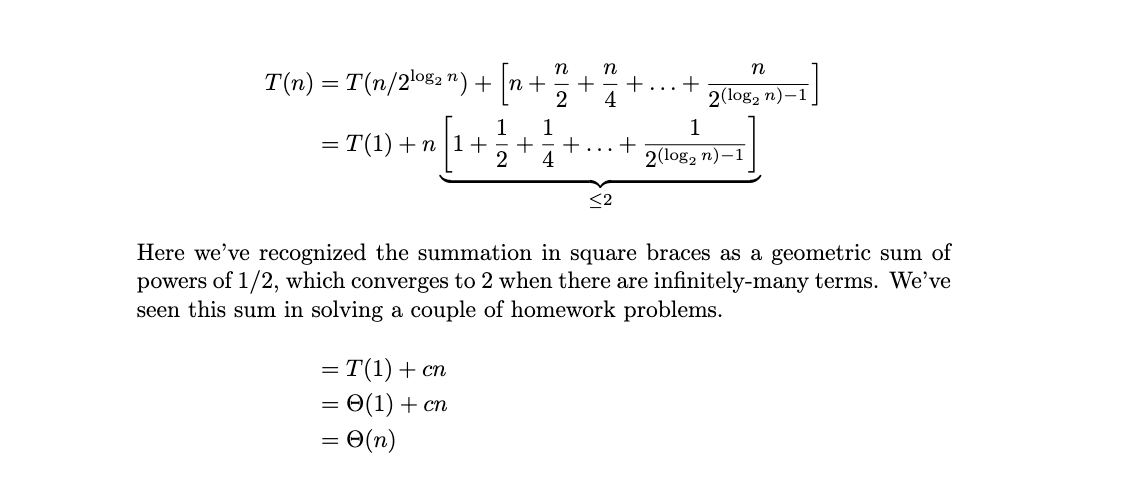
\includegraphics[width=.1\textwidth]{plot2.png}

    \end{soln}
\end{prob}
